\documentclass[man]{apa7}
\usepackage[spanish,es-nodecimaldot]{babel}
\usepackage{csquotes}
\usepackage{graphicx}
\usepackage{booktabs}
\usepackage{siunitx}
\usepackage{amsmath}
\usepackage{array}
\usepackage{float}
\usepackage{xcolor}
\usepackage{hyperref}
\usepackage{geometry}
\usepackage{mathptmx}
\usepackage{setspace}
\usepackage{caption}
\geometry{margin=2.5cm}
\setstretch{1.5}
\setlength{\tabcolsep}{4pt}
\renewcommand{\arraystretch}{1.1}
\captionsetup{font=small,labelfont=bf,skip=4pt}
\graphicspath{{../datos/punto2/Abtsgmuend_Untergroeningen/control_2_1/}{../datos/punto2/Abtsgmuend_Untergroeningen/extremos_2_2/}{../datos/punto2/Abtsgmuend_Untergroeningen/idf_2_3/}}

\begin{document}
\begin{titlepage}
\thispagestyle{empty}
\begin{center}
\vspace*{0.8cm}
% No se encontró un archivo del escudo en el repositorio. Colocar el archivo
% oficial en PUNTO_2/informe/escudo_unal.png para activarlo sin modificar el diseño.
\IfFileExists{escudo_unal.png}{\includegraphics[height=2.7cm]{escudo_unal.png}\\[0.65cm]}{\vspace*{2.7cm}}
{\bfseries UNIVERSIDAD NACIONAL DE COLOMBIA}\par
\vspace{1.25cm}
{\bfseries Tarea 2 de Hidrología:\par
Evapotranspiración y diseño hidrológico}\par
\vspace{1.15cm}
{\bfseries Andrés Francisco Idrobo Hidrobo — ID. 1089568711}\par
Facultad de Minas — Ingeniería Civil\par
\vspace{0.55cm}
{\bfseries Enmaly Aleli Manturano Grajeda — ID. 125817023}\par
Facultad de Minas — Ingeniería Geológica\par
\vspace{0.55cm}
{\bfseries Jeyson Cristian Javier Irpanoca — ID. 125496042}\par
Facultad de Minas — Ingeniería Geológica\par
\vspace{1.15cm}
Asignatura: Hidrología\par
Docente: Carlos David Hoyos\par
\vspace{0.9cm}
Fecha de entrega: 24 de noviembre de 2026
\end{center}
\end{titlepage}

\begin{abstract}
Este informe presenta el análisis del punto 2 de la Tarea 2 para la estación pluviométrica DWD 00020, Abtsgmünd--Untergröningen (Alemania). Se utilizaron datos de precipitación cada 10 minutos, un modelo digital de elevación SRTM, ESA WorldCover 2021 y la referencia KOSTRA-DWD-2020. Se documentan el control de calidad, el análisis de extremos, las curvas IDF, el diseño preliminar de una alcantarilla y un tanque de detención, la incertidumbre Monte Carlo y la bonificación Peaks Over Threshold. El outlet empleado es sintético y se deriva del MDE; esta limitación y el riesgo residual se declaran explícitamente.
\end{abstract}

\section{Espacio reservado para el punto 1}
\textbf{Esta sección debe ser completada por los integrantes responsables del punto 1.} Debe incorporarse aquí el análisis de la cuenca de la Tarea 1, incluyendo delimitación, precipitación, caudales, temperatura, climatología, tendencias, metodología, resultados y conclusiones.\par

Como referencia de los datos del grupo, la Tarea 1 trabajó con la cuenca PE\_200907 (Racarumi, Chancay--Lambayeque), ubicada aproximadamente en $-6.633^\circ$ N y $-79.317^\circ$ W, con área de \SI{2363.302}{km^2}. Los productos originales se conservan en `../PUNTO_1/datos/punto1/` y no se sustituyen por los datos independientes usados en este punto 2.

\newpage
\section{Punto 2: análisis hidrológico independiente}
\subsection{Objetivos y alcance}
El objetivo es caracterizar extremos de precipitación subdiaria y emplearlos en el diseño preliminar de obras de drenaje. El punto 2 es independiente del punto 1; por ello se seleccionó la estación DWD 00020, cuya serie histórica satisface la resolución temporal requerida.

\subsection{Datos y control de calidad (2.1)}
La estación Abtsgmünd--Untergröningen se ubica en Alemania y dispone de precipitación cada 10 minutos entre 2004 y 2025. Se conservaron los datos originales, metadatos, códigos de calidad y una serie procesada reproducible. Los valores faltantes y códigos inválidos se transformaron en datos ausentes; no se imputaron sin una decisión metodológica explícita. La serie se auditó por intervalos temporales, cobertura mensual y año hidrológico.

La cuenca sintética fue delimitada sobre el MDE SRTM. Su área es \SI{0.123154}{km^2}; la longitud del cauce principal es \SI{382.69}{m} y su pendiente media es \SI{0.1254}{m/m}. La estación queda fuera del polígono de drenaje, por lo que representa la lluvia regional y no un punto de aforo dentro de la microcuenca.

\begin{figure}[H]
\centering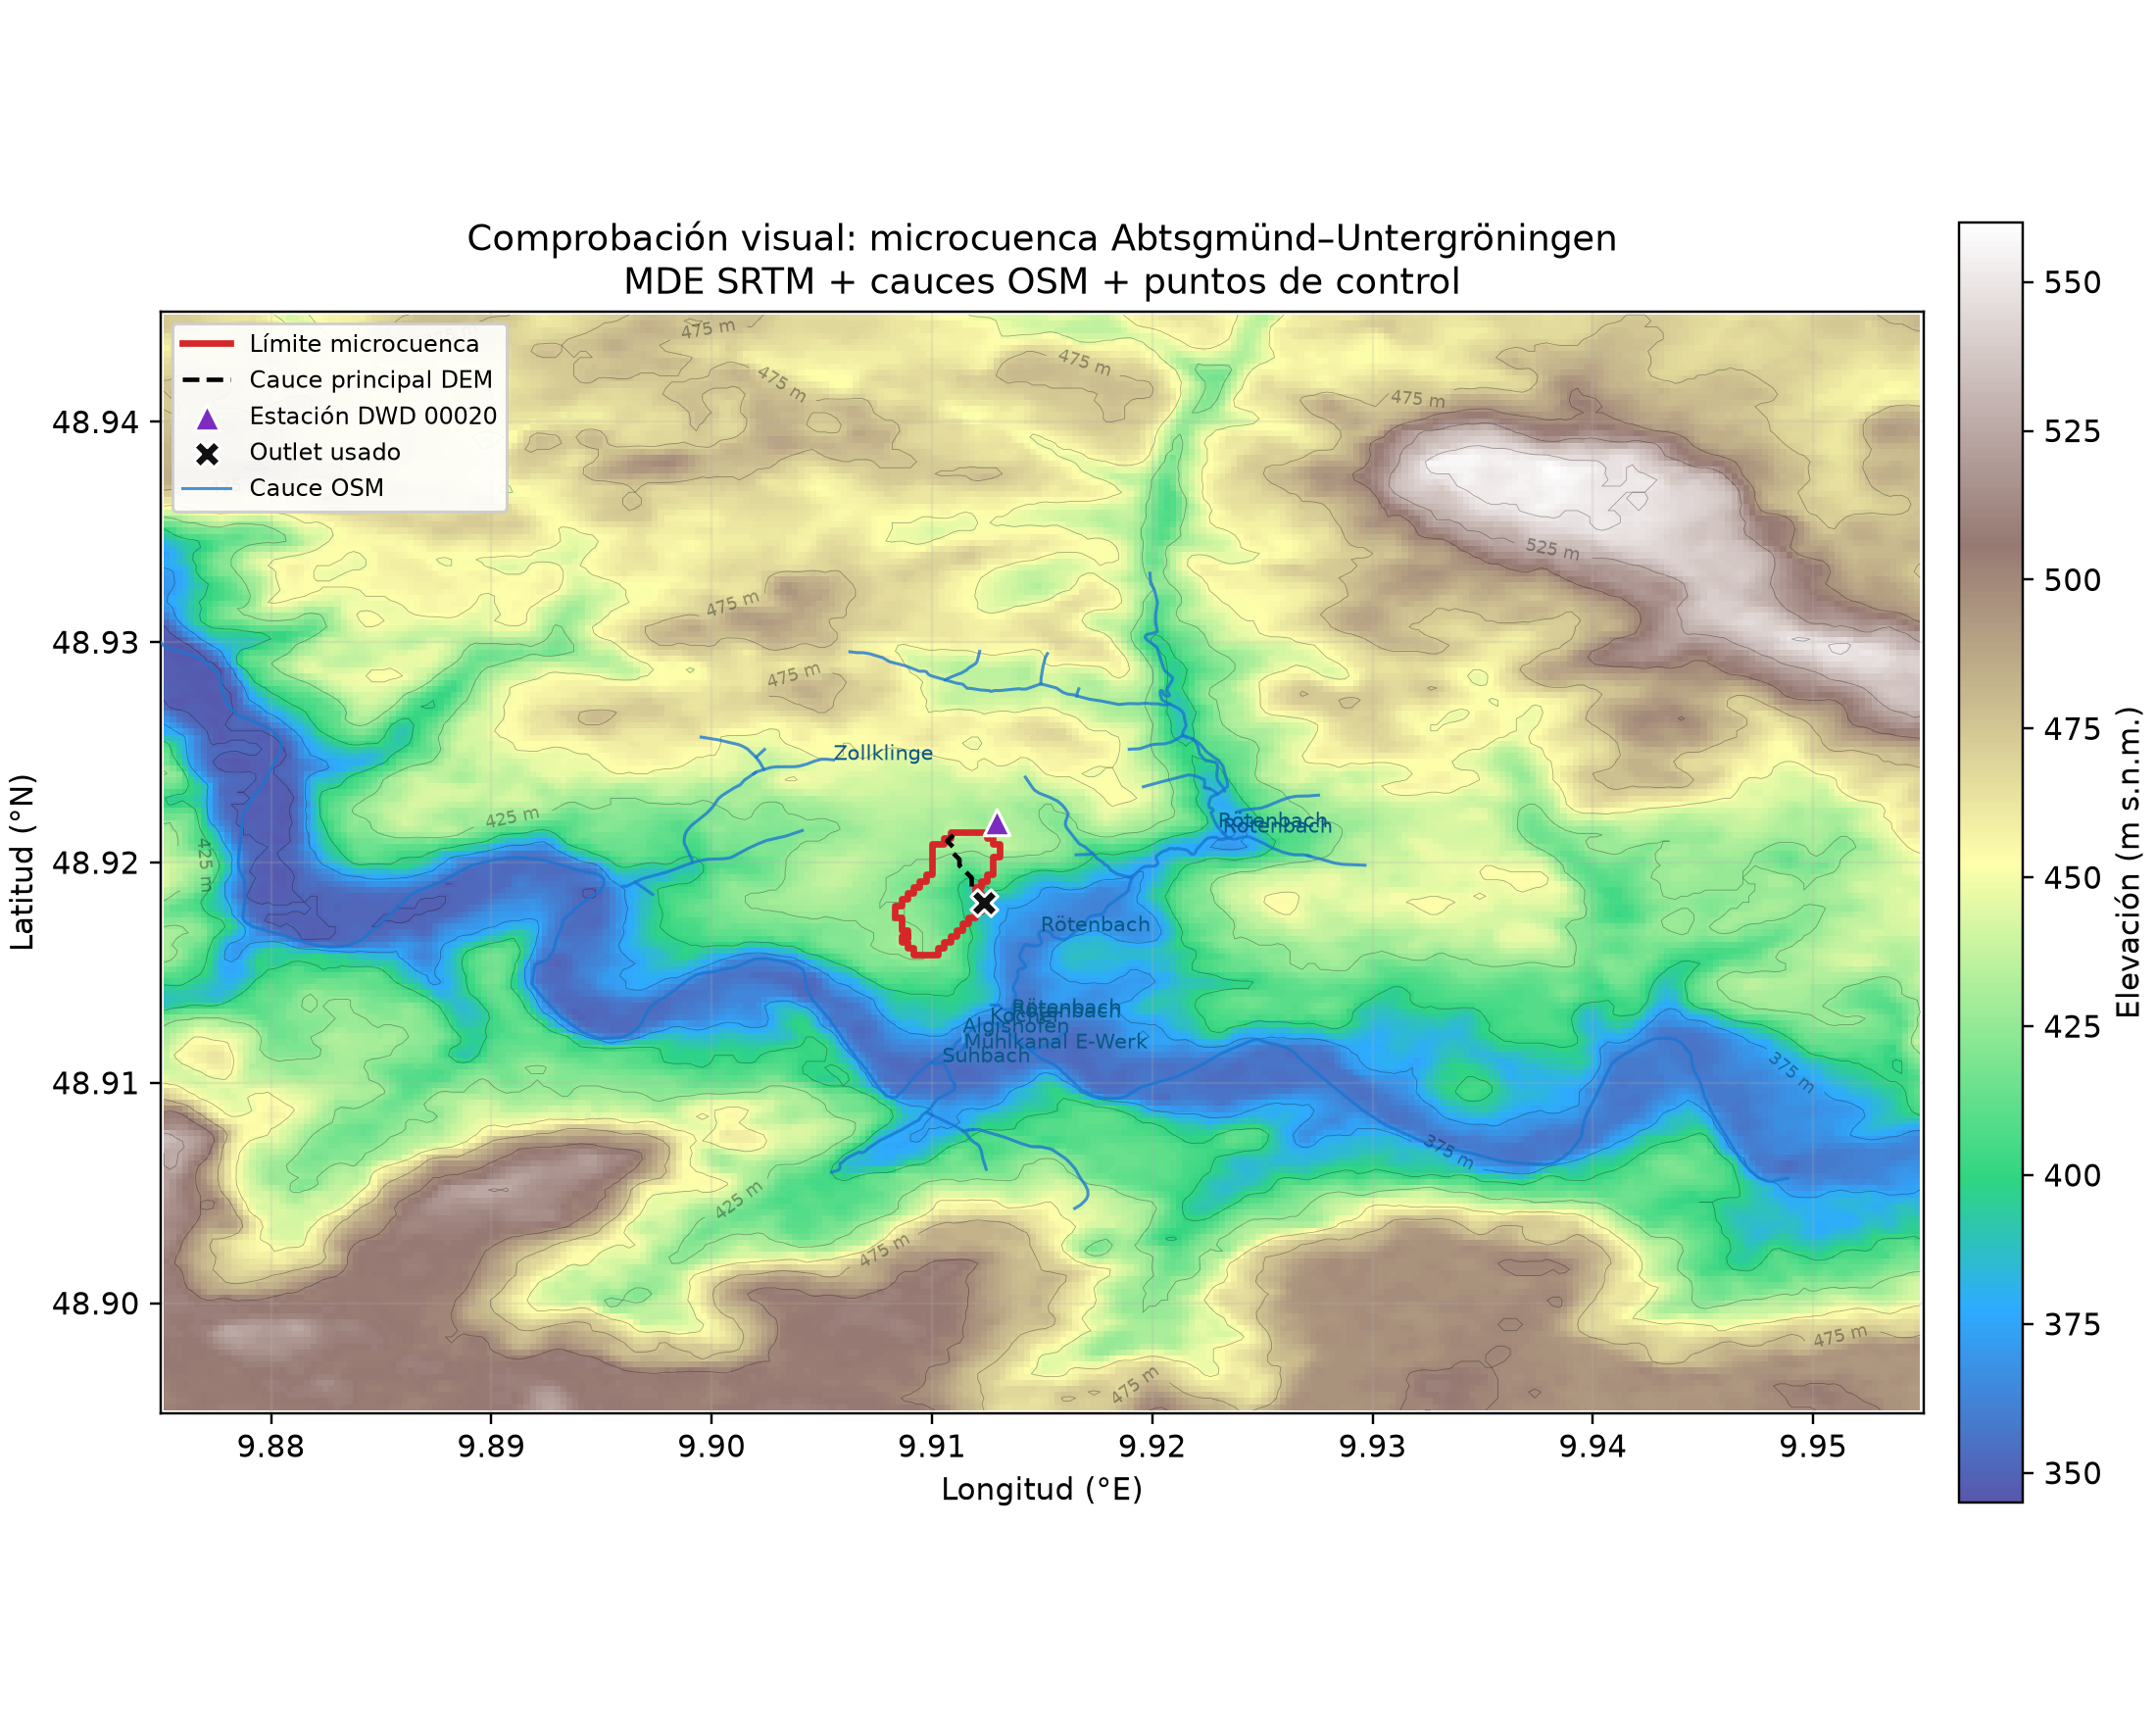
\includegraphics[width=0.92\linewidth]{mapa_revision_visual.png}
\caption{Contexto topográfico, límite de microcuenca, estación, outlet y cauces cartografiados.}
\label{fig:mapa}
\end{figure}

\subsection{Extremos y distribuciones (2.2)}
Se construyeron máximos anuales hidrológicos para duraciones de 10 minutos a 24 horas. Se compararon Gumbel, GEV y Log-Pearson III mediante momentos, L-momentos y máxima verosimilitud. Las pruebas Kolmogorov--Smirnov y Cramér--von Mises, junto con los gráficos de probabilidad, condujeron a seleccionar GEV por máxima verosimilitud como modelo de referencia. La selección es estadística y no implica que el modelo sea una representación física perfecta.

El bootstrap de cuantiles muestra incertidumbre creciente para periodos de retorno altos y duraciones largas. En 12--24 horas aparecen intervalos muy amplios, por lo que esas extrapolaciones deben interpretarse con cautela. Las pruebas de Kendall no detectaron tendencias significativas al 5\%; esto se expresa como ``no se detectó tendencia'', no como garantía de estacionariedad futura.

\begin{figure}[H]
\centering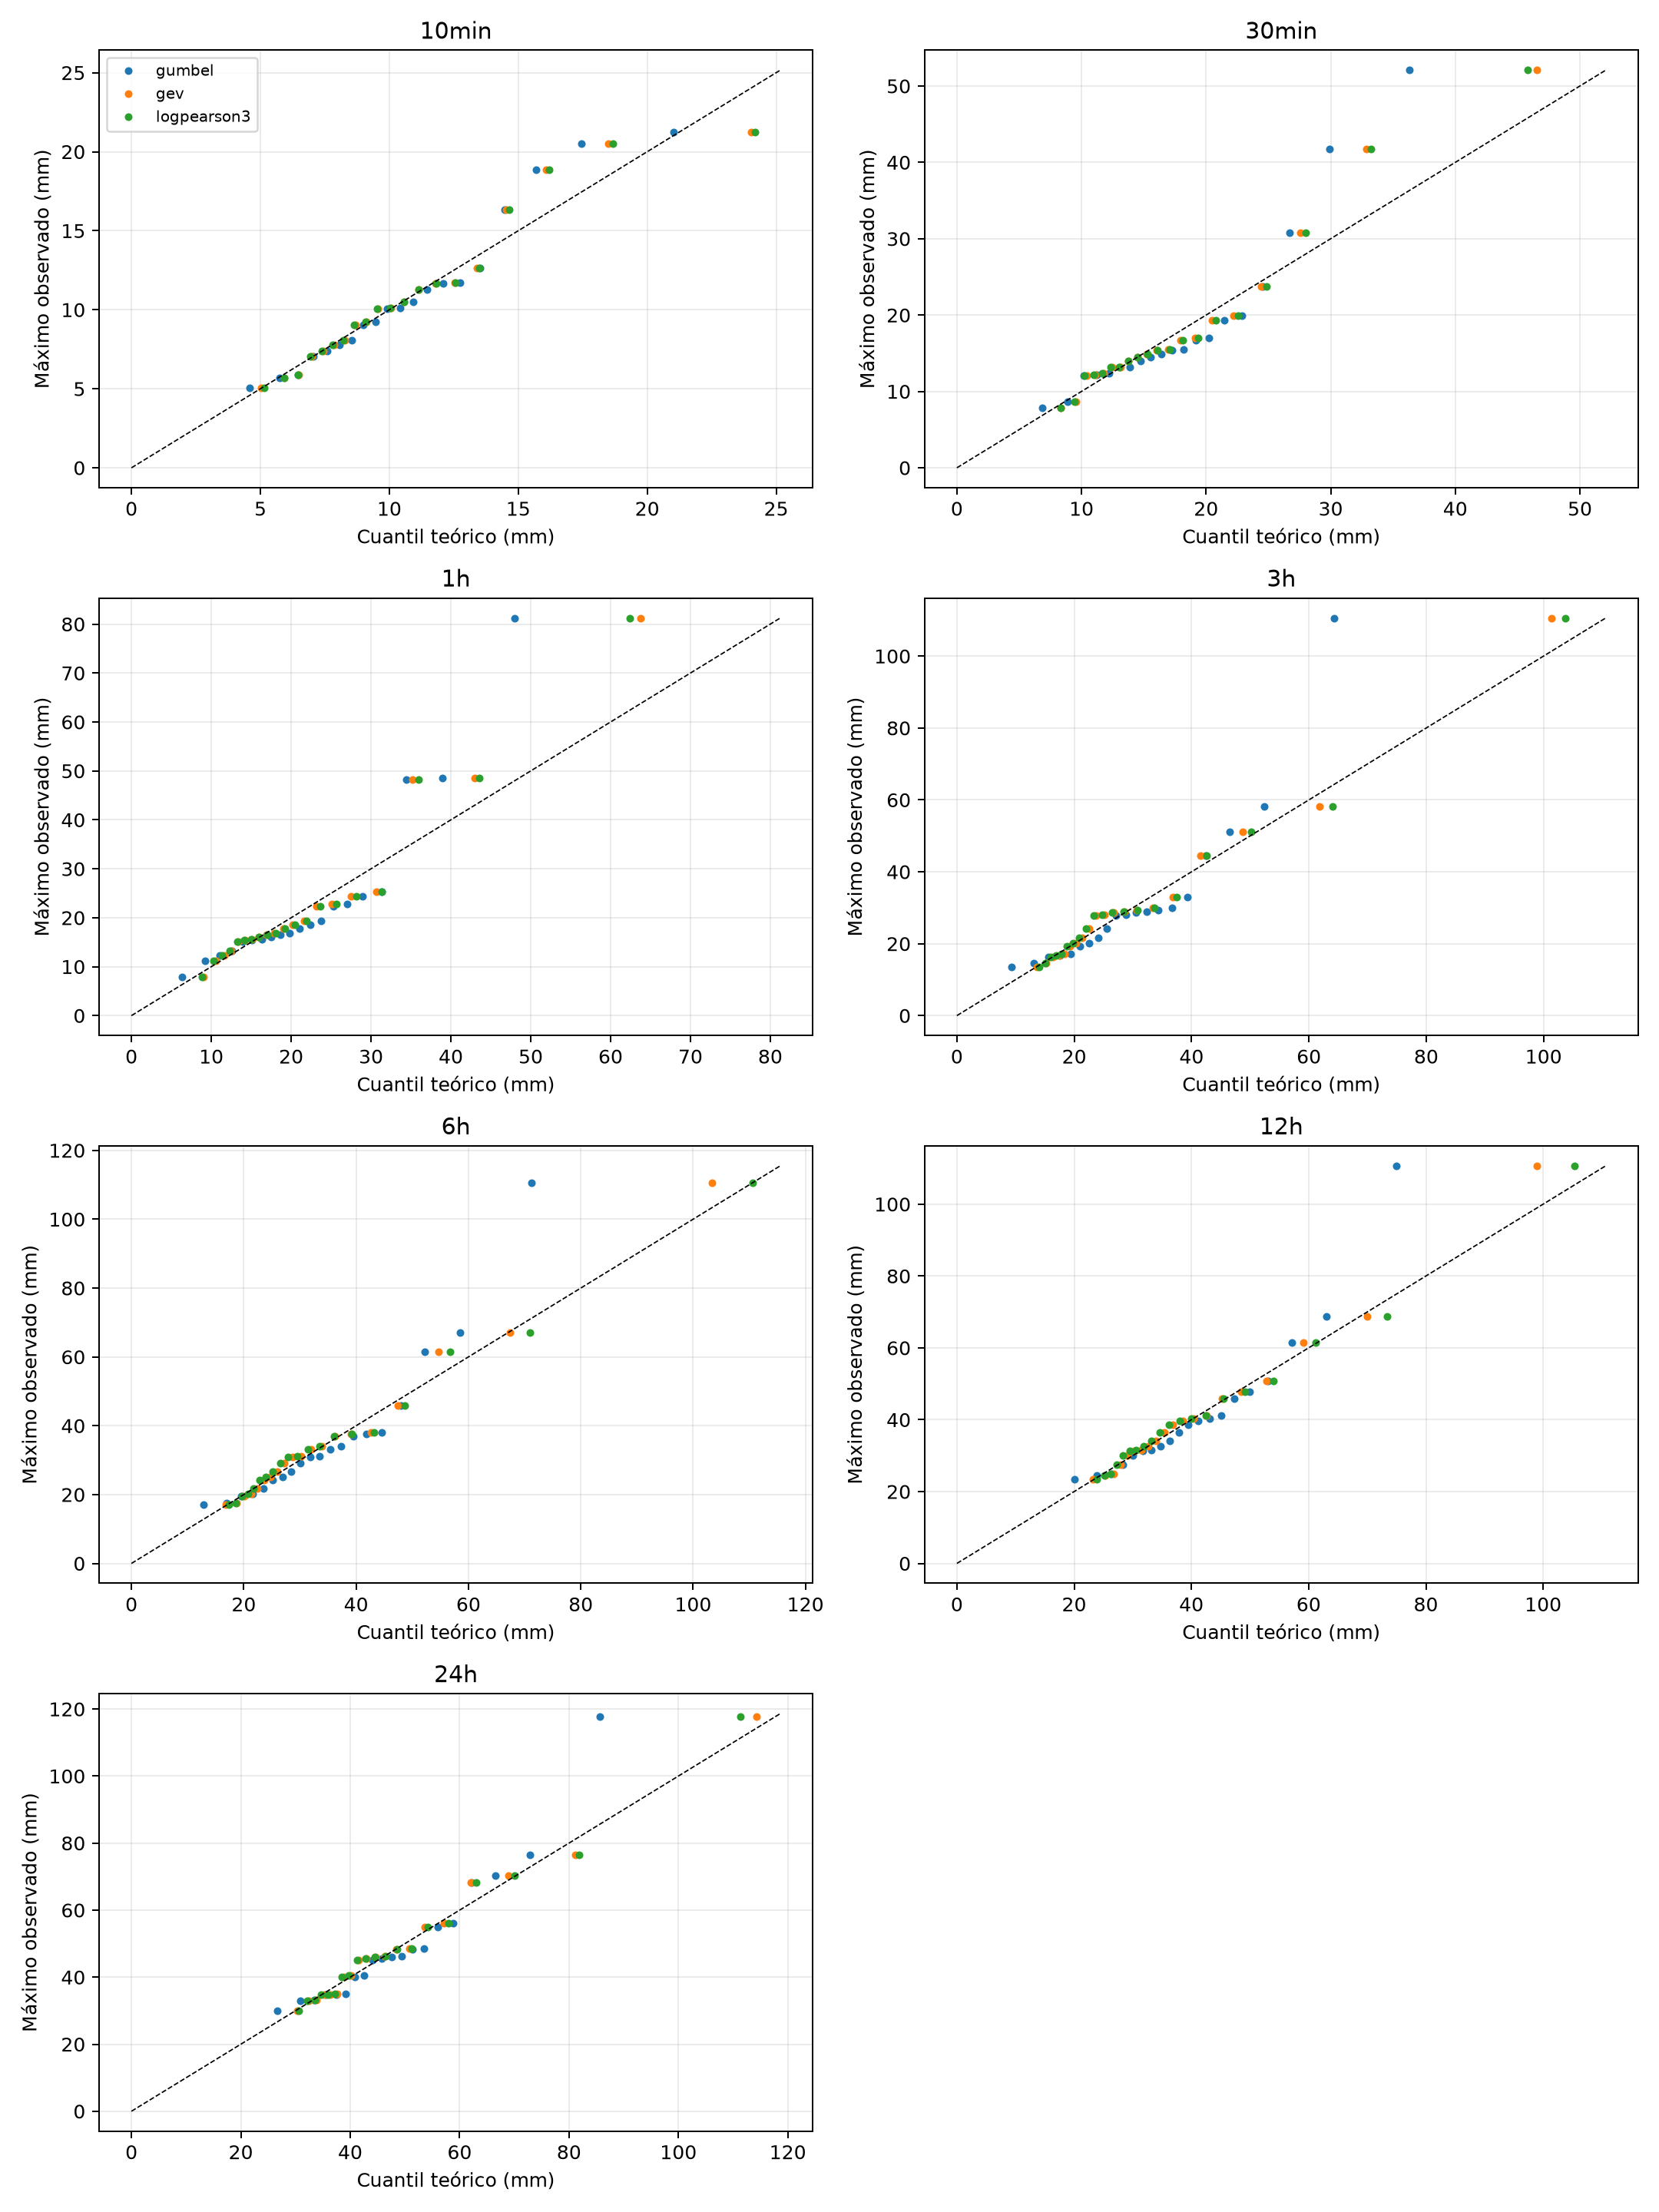
\includegraphics[width=0.95\linewidth]{graficas_probabilidad_2_2.png}
\caption{Gráficos de probabilidad para las distribuciones evaluadas.}
\end{figure}

\subsection{Curvas IDF y comparación externa (2.3)}
La IDF local se construyó con GEV-MLE. Las intensidades aumentan al disminuir la duración y al aumentar el periodo de retorno. La comparación con KOSTRA-DWD-2020 muestra que la curva local es similar o inferior para retornos cortos, pero más severa en varios escenarios de retorno alto; para 1 hora y $T=100$ años el cociente local/KOSTRA es aproximadamente 2.03, y para 6 horas es aproximadamente 2.08.

El máximo de 1 hora del año hidrológico 2021 fue \SI{48.27}{mm}, con periodo de retorno GEV-MLE aproximado de 17.4 años. Este evento no se interpreta por sí solo como evidencia de cambio climático.

\begin{figure}[H]
\centering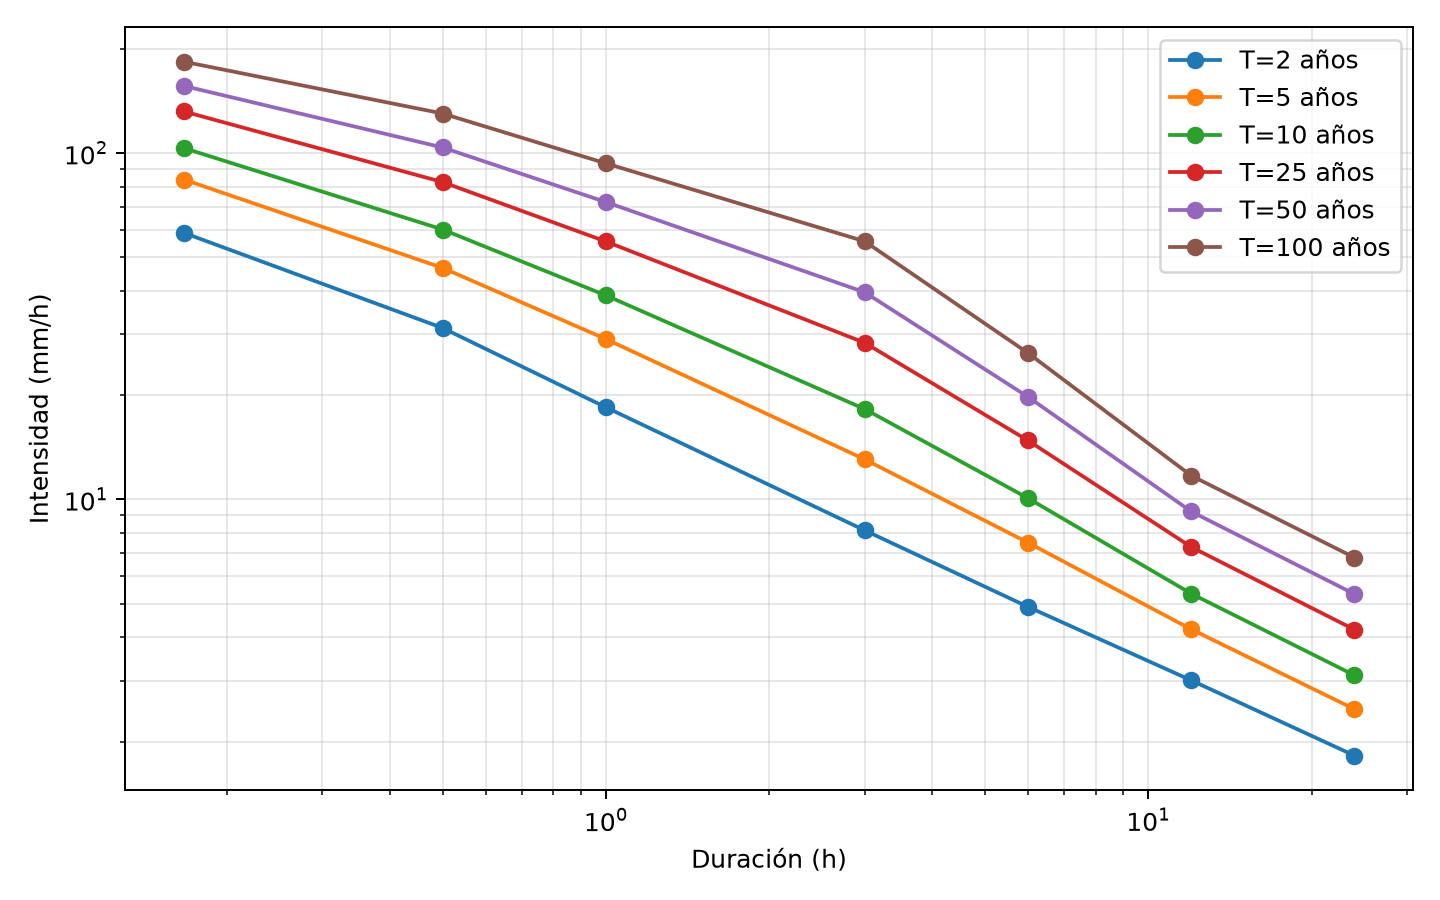
\includegraphics[width=0.86\linewidth]{idf_gev_mle.png}
\caption{Curvas IDF basadas en GEV-MLE.}
\end{figure}

\subsection{Diseño de alcantarilla y tanque (2.4)}
\subsubsection{Outlet y delimitación}
El outlet adoptado es $(48.9181944^\circ\ \mathrm{N},\ 9.9123611^\circ\ \mathrm{E})$. Coincide con el extremo aguas abajo del cauce principal derivado del MDE y queda dentro del polígono. La revisión con OpenStreetMap no encontró coincidencia exacta con una línea OSM; por tanto se declara como outlet sintético, no como obra existente ni punto de aforo real (véase la ampliación en la Figura~\ref{fig:detalle}).

\begin{figure}[H]
\centering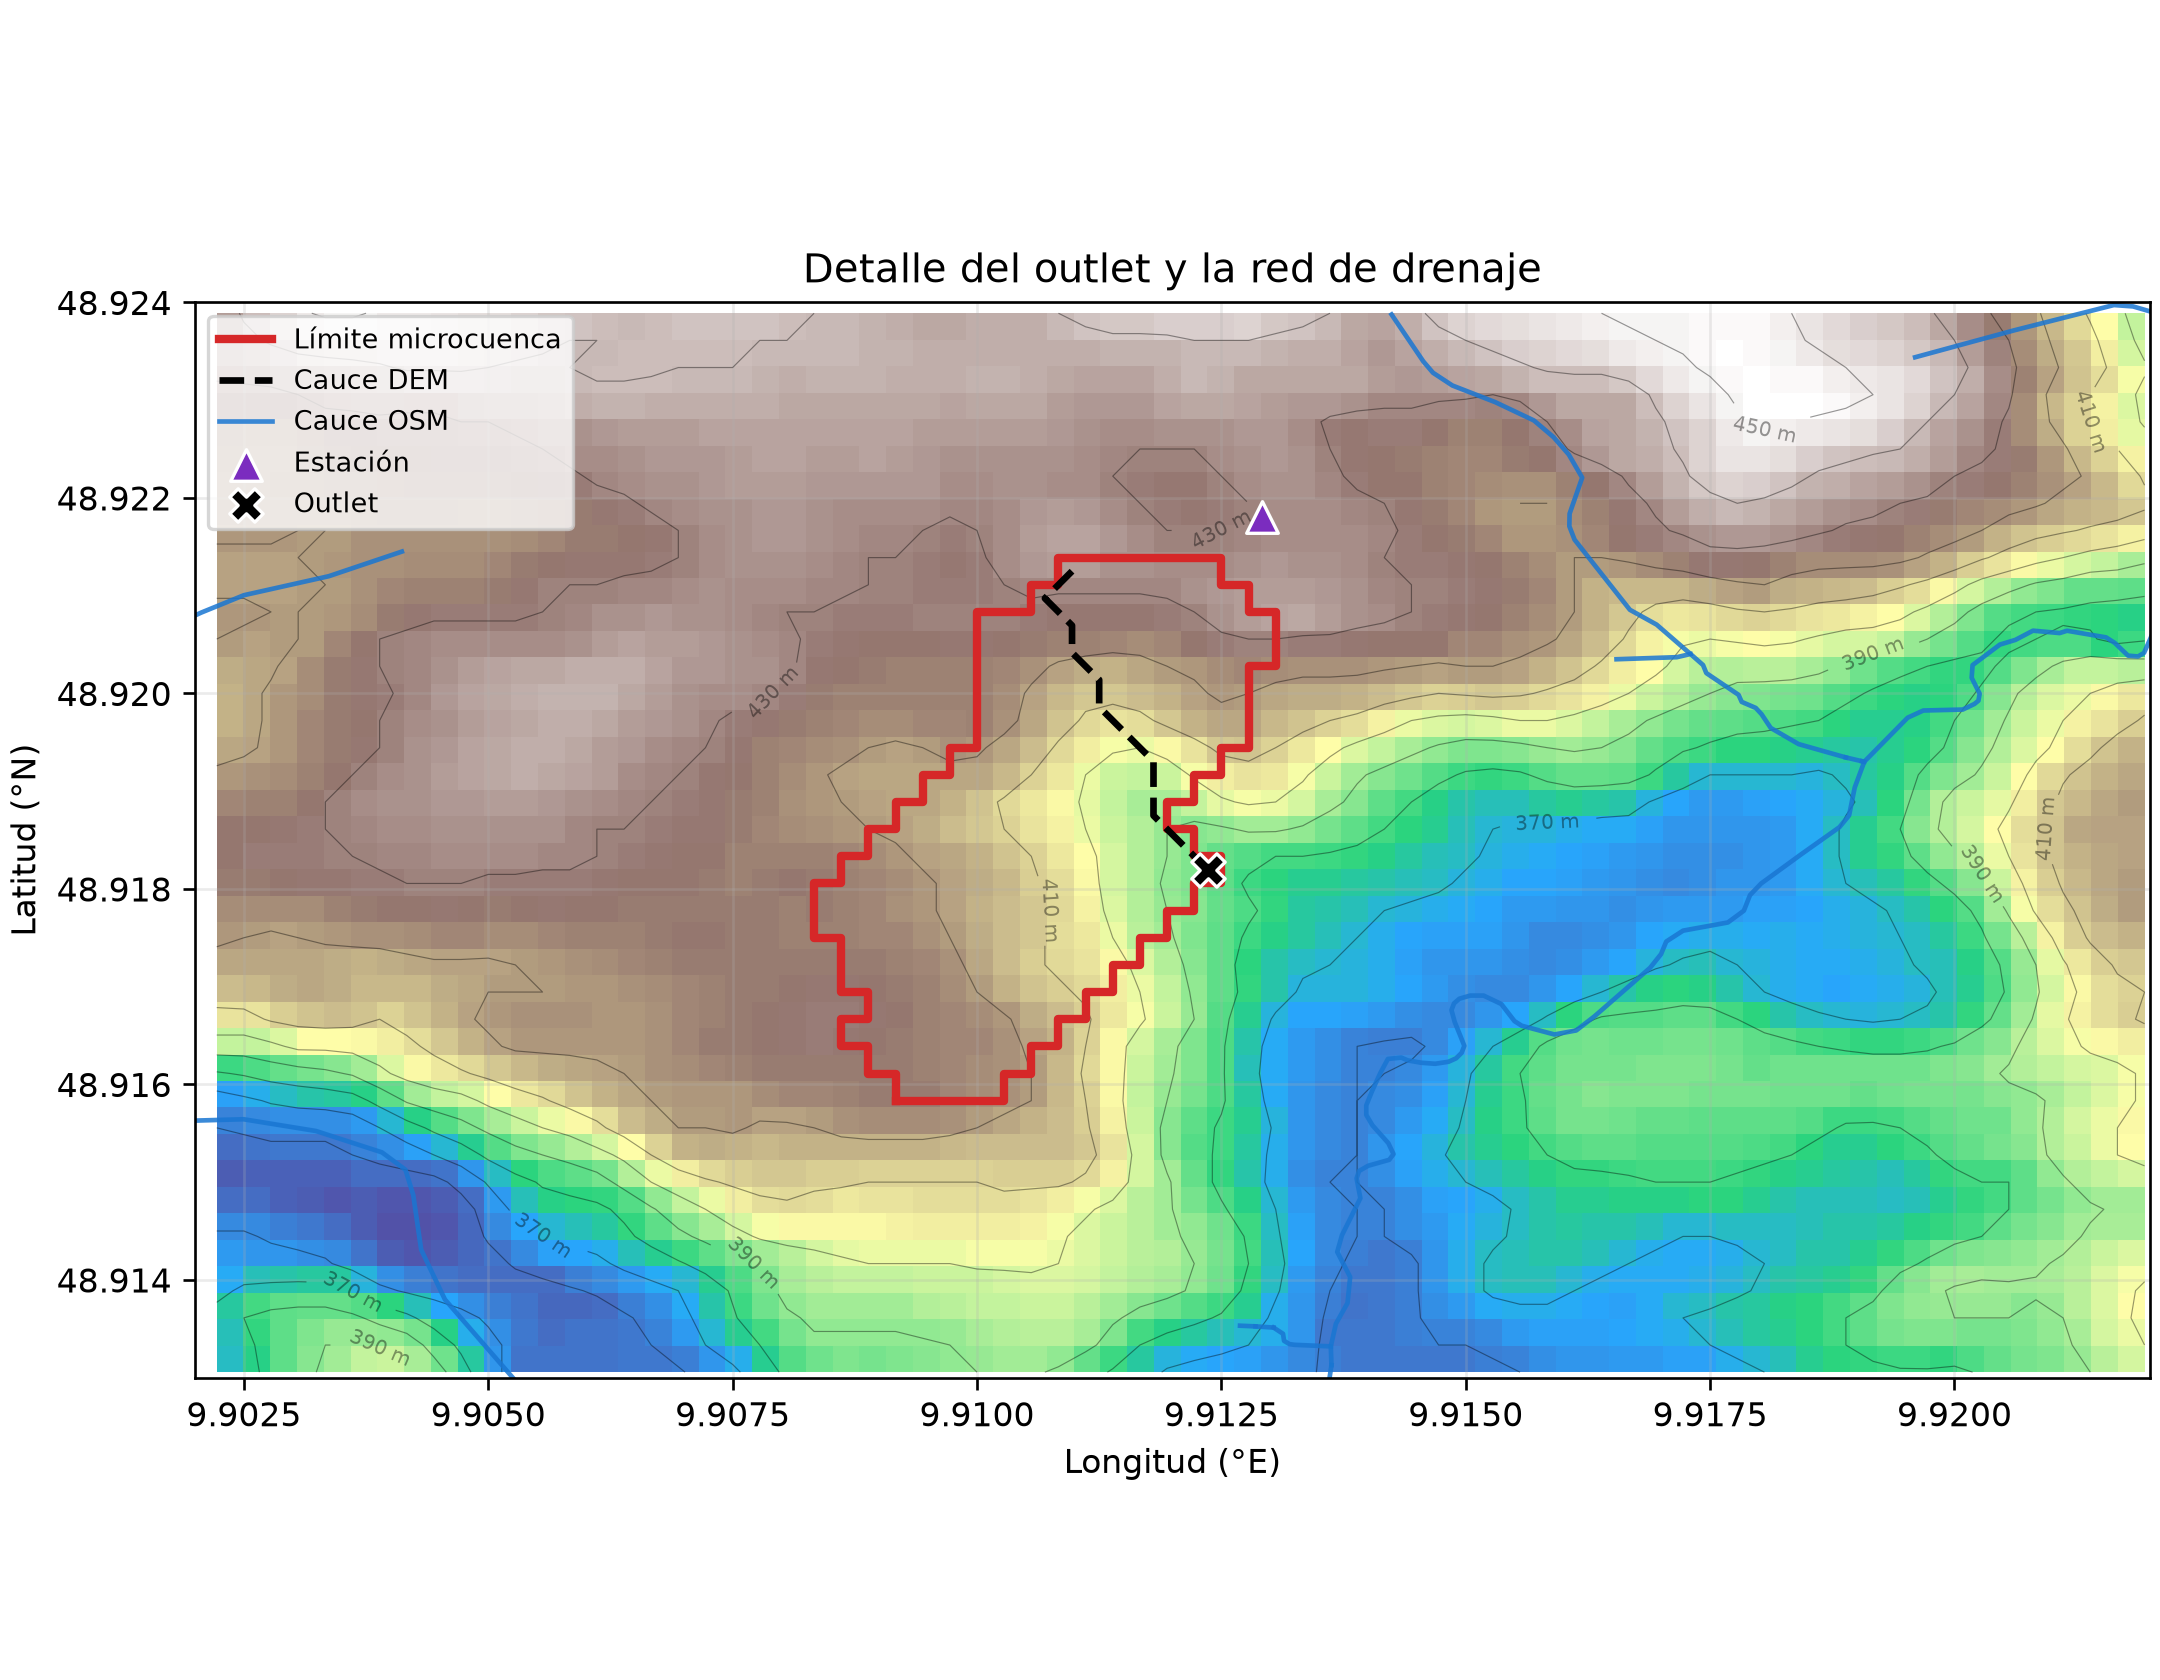
\includegraphics[width=0.9\linewidth]{mapa_revision_visual_detalle.png}
\caption{Detalle del outlet y comparación entre cauce DEM y geometrías OSM.}
\label{fig:detalle}
\end{figure}

\subsubsection{Método racional y alcantarilla}
La cobertura ESA WorldCover 2021 se resumió en árboles (56.17\%), pastizal (32.10\%) y cultivo (11.74\%). Con coeficientes de diseño 0.30, 0.35 y 0.45, respectivamente, se obtuvo $C=0.334$. Estos coeficientes son supuestos de ingeniería basados en Chow et al. (1988), no mediciones directas; se evaluó sensibilidad de $C=0.267$ a $C=0.400$.

Para $T=25$ años y el tiempo de concentración de Kirpich se obtuvo $Q_p=\SI{3.57}{m^3/s}$. La alcantarilla circular adoptada tiene diámetro \SI{1.50}{m}, pendiente \SI{0.010}{m/m}, Manning $n=0.013$ y capacidad \SI{7.08}{m^3/s}. El factor de seguridad respecto al caudal mediano es 1.98. El Monte Carlo estima falla anual de 0.82\% y riesgo acumulado de 21.9\% en 30 años; este riesgo residual no se presenta como riesgo bajo.

\subsubsection{Tanque de detención}
Se evaluaron hietogramas de 30, 60 y 90 minutos con tres posiciones del pico. El escenario crítico requiere \SI{1019.15}{m^3} y alcanza \SI{1.93}{m} de profundidad. El tanque rectangular propuesto mide $24\times22$ m, tiene \SI{2.0}{m} de profundidad útil y \SI{0.5}{m} de borde libre, para un volumen útil de \SI{1056}{m^3}. El margen volumétrico es \SI{36.85}{m^3}.

\subsection{Bonificación POT (2.5)}
Se aplicó Peaks Over Threshold a acumulados horarios derivados de la serie de 10 minutos. Con umbral P95 (\SI{0.530}{mm/h}) y declustering de 24 horas se obtuvieron 1523 picos y una tasa de 71.22 eventos/año. La Generalizada de Pareto produjo \SI{56.35}{mm} para 1 hora y $T=100$ años. La sensibilidad P90--P98 varió entre \SI{52.87}{mm} y \SI{61.10}{mm}; la GEV-MLE da \SI{93.36}{mm} para el mismo escenario. POT se conserva como análisis complementario y no sustituye la IDF principal.

\section{Discusión integrada y limitaciones}
La recomendación depende de la IDF GEV-MLE, del outlet sintético, del coeficiente $C$, del tiempo de concentración y de los supuestos de Manning y tránsito. La mayor incertidumbre aparece en la extrapolación de retornos largos y en la representación espacial del outlet. Cambios en cobertura o humedad antecedente modificarían $C$ y, por tanto, el caudal racional. El riesgo efectivo de 21.9\% a 30 años debe guiar una eventual medida adicional de seguridad, como mayor diámetro, alivio de emergencia o control operativo.

\section{Reproducibilidad y declaración de uso de IA}
Los datos procesados, scripts y resultados se encuentran en `../datos/punto2/`, `../codigo/punto2/` y `../productos/punto2/`. La auditoría previa obtuvo 10/10 controles OK. La asistencia de IA se utilizó para organizar código, revisar consistencia, generar mapas estáticos y redactar borradores; las decisiones metodológicas, revisión de resultados y responsabilidad académica corresponden al grupo.

\section{Conclusiones}
La estación DWD 00020 permite un análisis subdiario reproducible. La GEV-MLE se seleccionó como distribución de referencia y la comparación KOSTRA evidenció mayor severidad local en la cola. El diseño preliminar consta de una alcantarilla de \SI{1.50}{m} y un tanque de \SI{1056}{m^3}, con riesgo residual explícito. POT confirma la sensibilidad del análisis de extremos, pero no reemplaza la IDF principal. La interpretación debe conservar la limitación del outlet sintético.

\begin{flushleft}
\textbf{Referencias}\par
Chow, V. T., Maidment, D. R., \& Mays, L. W. (1988). \textit{Applied hydrology}. McGraw--Hill.\\
Deutscher Wetterdienst. (2026). \textit{Datos históricos de precipitación de la estación 00020}.\\
European Space Agency. (2021). \textit{ESA WorldCover 10 m 2021}.\\
OpenStreetMap contributors. (2026). \textit{OpenStreetMap}. \url{https://www.openstreetmap.org/}\\
SRTM. (2013). \textit{Shuttle Radar Topography Mission global digital elevation model}. NASA.
\end{flushleft}

\end{document}
